\documentclass[10pt,a4paper]{article}

\usepackage[T1]{fontenc}
\usepackage[a4paper,margin=1.35cm]{geometry}
\usepackage{graphicx}
\usepackage{xcolor}
\usepackage{tikz}

\usetikzlibrary{arrows.meta, positioning, calc, shapes.misc}

\definecolor{lavagna}{RGB}{36,93,130}
\definecolor{utente}{RGB}{37,125,93}
\definecolor{lightblue}{RGB}{235,243,249}
\definecolor{lightgreen}{RGB}{236,247,241}
\definecolor{lightyellow}{RGB}{250,244,226}
\definecolor{lightred}{RGB}{251,235,235}
\definecolor{border}{RGB}{55,62,70}

\pagestyle{empty}
\setlength{\parindent}{0pt}
\setlength{\parskip}{1em}
\setlength{\emergencystretch}{4em}
\linespread{1}

\makeatletter
\renewcommand\section{\@startsection{section}{1}{0pt}{1em}{1em}{\normalfont\large\bfseries}}
\makeatother

\tikzset{
    box/.style={
        rectangle,
        rounded corners=2pt,
        draw=border,
        line width=0.45pt,
        align=center,
        inner sep=3.2pt,
        minimum height=8mm
    },
    state/.style={
        rounded rectangle,
        draw=border,
        line width=0.45pt,
        fill=lightblue,
        align=center,
        inner sep=3pt,
        minimum width=27mm,
        minimum height=8mm
    },
    lblnofill/.style={
    font=\sffamily\scriptsize,
    align=center,
    inner sep=1pt
    },
    arrow/.style={-{Latex[length=2mm]}, line width=0.45pt},
    dottedarrow/.style={-{Latex[length=2mm]}, line width=0.45pt, dashed}
}



\begin{document}

\begin{center}
{\Large\bfseries Documentazione Progetto di Reti Informatiche A.A. 2025/2026}
\\\Large Daniele Pisani
\end{center}

\section{Scelte implementative riguardo la comunicazione}

La comunicazione fra lavagna e utenti avviene tramite protocollo TCP su \texttt{127.0.0.1}, con la lavagna che si posiziona sulla porta \texttt{5678} e gli utenti sulle porte successive, dalla \texttt{5679} in poi. Inoltre utilizzo TCP anche per la parte P2P, per la quale ogni utente inizializza un server P2P da usare per comunicare con gli altri utenti. La scelta di usare TCP deriva dal fatto che l'utilizzo di UDP avrebbe aggiunto notevole complessità al progetto. Avrebbe infatti richiesto di gestire gli errori di consegna dei pacchetti e, specialmente nel P2P, sarebbe stato necessario introdurre meccanismi per evitare che la perdita di un messaggio \texttt{CHOOSE\_USER} bloccasse la selezione del vincitore della card, quali per esempio l'introduzione di un quorum o di una gestione delle ritrasmissioni.

Le connessioni multiple vengono gestite dalla lavagna tramite multiplexing usando \texttt{select()}, mentre il processo utente usa un approccio misto. Il thread principale gestisce la connessione con la lavagna e l'input da terminale, un secondo thread ascolta i messaggi P2P dagli altri utenti e un worker separato simula l'esecuzione della card vinta. Questa scelta isola meglio i compiti del processo utente e permette di rispondere ai comandi ricevuti da lavagna o terminale e di ricevere i costi P2P in qualsiasi momento, anche mentre si attende l'elaborazione di una carta.

Per scambiare messaggi viene usato un formato binario standard per costituire l'header, composto da: 32 bit per il tipo del messaggio e 32 bit per la lunghezza del payload, entrambi in network byte order. Molti messaggi, come \texttt{PING\_USER}, \texttt{PONG\_LAVAGNA} e \texttt{QUIT}, non hanno payload. Gli altri messaggi possiedono un payload di dimensioni variabili, che può contenere sia altri byte di campi relativi al messaggio, sia eventuali stringhe terminate da \texttt{\textbackslash 0}. Ho adottato questa soluzione in quanto mi sembrava efficiente per costruire e leggere velocemente i pacchetti necessari per il progetto, spesso utilizzati per trasmettere informazioni numeriche, gestendo le stringhe specificamente solo quando richiesto.  

\section{Struttura logica del programma}

Ho cercato di strutturare il programma in modo modulare. I moduli \texttt{server} e \texttt{client} astraggono la gestione dei socket, mentre \texttt{protocol} contiene la logica comune di serializzazione e deserializzazione dei messaggi. In questo modo sia la lavagna centrale sia il server P2P degli utenti usano la stessa API di basso livello, evitando così di avere duplicati del codice di accettazione, lettura e invio dei messaggi.

La lavagna e l'utente hanno poi due strutture parallele per mantenere lo stato. La lavagna utilizza un \texttt{Database} statico con array di utenti e card; gli array hanno dimensione fissa, rispettivamente \texttt{MAX\_USERS} e \texttt{MAX\_CARDS}. Non e' una struttura ottima ne' dal punto di vista algoritmico ne' dal punto di vista della memoria; tuttavia, essendo l'ambito del progetto limitato, ho preferito un'implementazione semplice basata su array che non introducesse troppa complessità nella gestione della memoria. Si potrebbe pensare con future ottimizzazioni di gestire dinamicamente lo spazio utilizzato e ottimizzare le operazioni di estrazione di elementi necessarie al funzionamento del progetto. L'utente invece mantiene una struttura globale \texttt{Utente}, incapsulata nel modulo \texttt{utente\_state.c}: gli altri moduli non vi accedono direttamente, ma devono usare le funzioni esposte dall'API. Inoltre le parti mutabili condivise tra i thread dell'utente sono protette da mutex.

L'utente infine è strutturato per avere due thread oltre al principale, oltre al thread per gestire i messaggi del server P2P utilizza infatti anche un worker thread. Quando un utente vince una card, invia \texttt{ACK\_CARD} alla lavagna, entra nello stato di lavoro e avvia il worker. Il worker non comunica con l'esterno, si limita a simulare il tempo di esecuzione e a segnalare allo stato condiviso quando la card puo' essere completata. Il thread principale una volta notificato, cambia lo stato e invia \texttt{CARD\_DONE} alla lavagna.

\newpage
\begin{center}
\textbf{Grafico della memoria del progetto}
\vspace{1em}

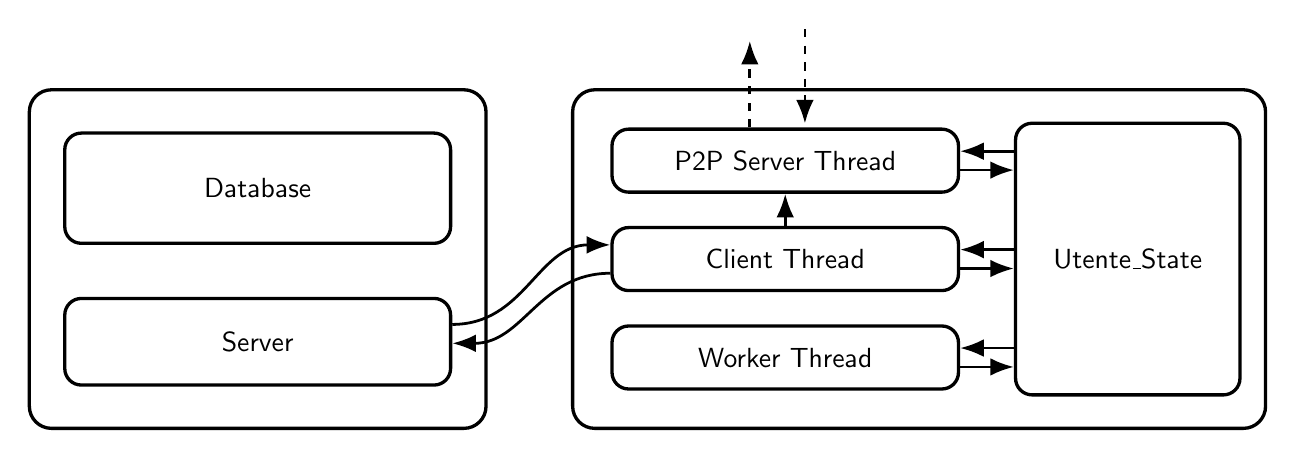
\begin{tikzpicture}[
    font=\sffamily,
    box/.style={
        draw,
        rounded corners=6pt,
        line width=1.2pt,
        align=center,
        minimum height=1cm
    },
    bigbox/.style={
        draw,
        rounded corners=8pt,
        line width=1.2pt
    },
    arrow/.style={
        -{Latex[length=3mm]},
        line width=1pt
    },
    dashedarrow/.style={
        dashed,
        -{Latex[length=3mm]},
        line width=1pt
    }
]

% =========================
% Contenitore sinistro
% =========================
\node[bigbox, minimum width=5.8cm, minimum height=4.3cm] (leftcontainer) at (0,0) {};

\node[box, minimum width=4.9cm, minimum height=1.4cm] (database)
    at ($(leftcontainer.center)+(0,0.9)$) {Database};

\node[box, minimum width=4.9cm, minimum height=1.1cm] (server)
    at ($(leftcontainer.center)+(0,-1.05)$) {Server};

% =========================
% Contenitore destro
% =========================
\node[bigbox, minimum width=8.8cm, minimum height=4.3cm] (rightcontainer) at (8.4,0) {};

\node[box, minimum width=4.4cm, minimum height=0.8cm] (p2p)
    at ($(rightcontainer.center)+(-1.7,1.25)$) {P2P Server Thread};

\node[box, minimum width=4.4cm, minimum height=0.8cm] (client)
    at ($(rightcontainer.center)+(-1.7,0)$) {Client Thread};

\node[box, minimum width=4.4cm, minimum height=0.8cm] (worker)
    at ($(rightcontainer.center)+(-1.7,-1.25)$) {Worker Thread};

\node[box, minimum width=2.85cm, minimum height=3.45cm] (state)
    at ($(rightcontainer.center)+(2.65,0)$) {Utente\_State};

% =========================
% Frecce tra Server e Client Thread
% =========================

\draw[arrow]
    ($(server.east)+(0,0.22)$)
    to[out=0,in=180,looseness=1.05]
    ($(client.west)+(0,0.18)$);

\draw[arrow]
    ($(client.west)+(0,-0.18)$)
    to[out=180,in=0,looseness=1.05]
    ($(server.east)+(0,-0.02)$);

% =========================
% Freccia verticale Client -> P2P
% =========================
\draw[arrow]
    (client.north) -- (p2p.south);

% =========================
% Frecce tratteggiate sopra P2P Server Thread
% =========================
\draw[dashedarrow]
    ($(p2p.north)+(-0.45,0)$) -- ++(0,1.1);

\draw[dashedarrow]
    ($(p2p.north)+(0.25,1.25)$) -- ($(p2p.north)+(0.25,0.05)$);

% =========================
% Connessioni con User_State
% =========================

% Punti sulla parete sinistra di User_State,
% alla stessa altezza dei tre thread
\coordinate (stateP2P)    at (state.west |- p2p.east);
\coordinate (stateClient) at (state.west |- client.east);
\coordinate (stateWorker) at (state.west |- worker.east);

% P2P Server Thread <-> User_State
\draw[arrow]
    ($(stateP2P)+(0,0.12)$) -- ($(p2p.east)+(0,0.12)$);

\draw[arrow]
    ($(p2p.east)+(0,-0.12)$) -- ($(stateP2P)+(0,-0.12)$);

% Client Thread <-> User_State
\draw[arrow]
    ($(stateClient)+(0,0.12)$) -- ($(client.east)+(0,0.12)$);

\draw[arrow]
    ($(client.east)+(0,-0.12)$) -- ($(stateClient)+(0,-0.12)$);

% Worker Thread <-> User_State
\draw[arrow]
    ($(stateWorker)+(0,0.12)$) -- ($(worker.east)+(0,0.12)$);

\draw[arrow]
    ($(worker.east)+(0,-0.12)$) -- ($(stateWorker)+(0,-0.12)$);

\end{tikzpicture}

\vspace{1em}


I tre thread del processo utente comunicano attraverso la macchina a stati contenuta in \texttt{Utente\_State}. Ogni stato descrive quale parte del processo deve agire: in \texttt{IDLE} l'utente attende una card, in \texttt{CHOOSING} raccoglie i costi e stabilisce se il vincitore è lui o un peer, in \texttt{ACK\_PENDING} deve confermare la vittoria, in \texttt{WORKING} il worker sta lavorando e in \texttt{DONE\_PENDING} il completamento deve essere notificato alla lavagna.

\vspace{1em}
\textbf{Grafico degli stati del progetto}

\resizebox{1\textwidth}{!}{%
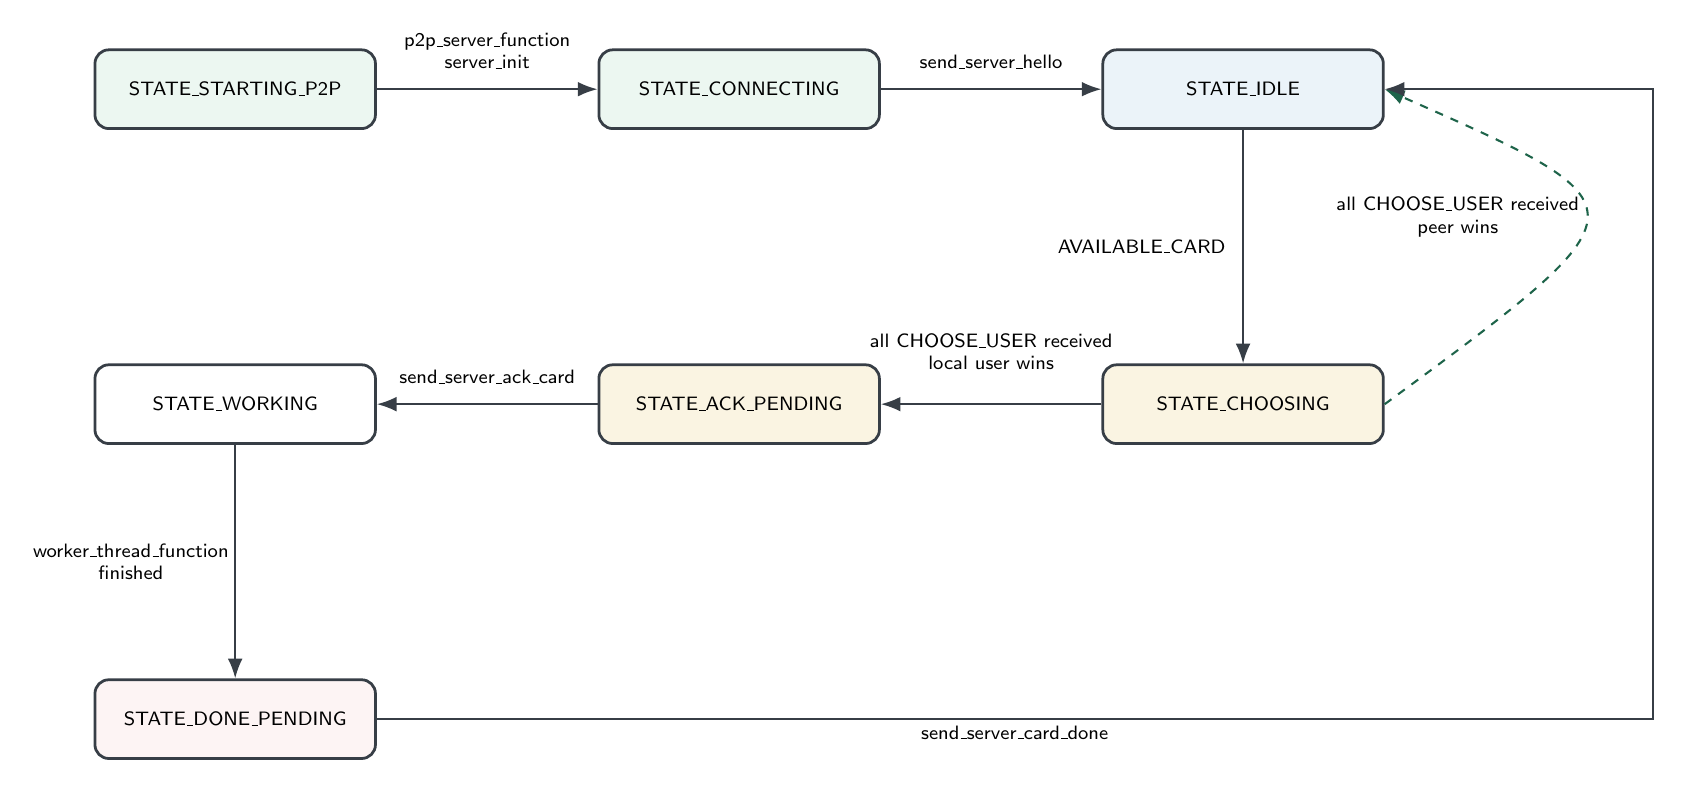
\begin{tikzpicture}[
    font=\sffamily,
    state/.style={
        draw=border,
        rounded corners=5pt,
        line width=1pt,
        minimum width=3.5cm,
        minimum height=1cm,
        text width=3cm,
        inner sep=8pt,
        align=center,
        font=\sffamily\scriptsize
    },
    setup/.style={state, fill=lightgreen},
    wait/.style={state, fill=lightblue},
    election/.style={state, fill=lightyellow},
    work/.style={state, fill=white},
    done_state/.style={state, fill=lightred!55},
    trans/.style={
        -{Latex[length=2.5mm]},
        line width=0.75pt,
        draw=border
    },
    alt/.style={trans, dashed, draw=utente!80!black},
    lbl/.style={
        font=\sffamily\scriptsize,
        align=center,
        inner sep=2pt,
        rounded corners=2pt
    }
]

\node[setup] (start) at (0,4) {STATE\_STARTING\_P2P};
\node[setup] (conn) at (6.4,4) {STATE\_CONNECTING};
\node[wait] (idle) at (12.8,4) {STATE\_IDLE};

\node[election] (choosing) at (12.8,0) {STATE\_CHOOSING};
\node[election] (ack) at (6.4,0) {STATE\_ACK\_PENDING};
\node[work] (working) at (0,0) {STATE\_WORKING};
\node[done_state] (done) at (0,-4) {STATE\_DONE\_PENDING};

\coordinate (returnB) at (18,-4);
\coordinate (returnC) at (18,4);

\draw[trans] (start.east) -- node[lbl, above=5pt] {p2p\_server\_function\\server\_init} (conn.west);
\draw[trans] (conn.east) -- node[lbl, above=5pt] {send\_server\_hello} (idle.west);
\draw[trans] (idle.south) -- node[lbl, left=4pt] {AVAILABLE\_CARD} (choosing.north);
\draw[alt] (choosing.east) .. controls (18,2.5) ..
    node[lbl, left, pos=0.5] {all CHOOSE\_USER received\\peer wins} (idle.east);
\draw[trans] (choosing.west) --
    node[lbl, above=10pt, pos=0.5, text width=3.4cm] {all CHOOSE\_USER received\\local user wins} (ack.east);
\draw[trans] (ack.west) -- node[lbl, above=5pt] {send\_server\_ack\_card} (working.east);
\draw[trans] (working.south) -- node[lbl, left] {worker\_thread\_function\\finished} (done.north);
\draw[trans] (done.east) -- node[lbl, below] {send\_server\_card\_done} (returnB)
    -- (returnC) -- (idle.east);

\end{tikzpicture}%
}
\end{center}

La state machine dell'applicazione utente si comporta a grandi linee come descritto in questo grafico. Sono presenti anche due ulteriori stati: \texttt{STATE\_DISCONNECTING} e \texttt{STATE\_SHUTTING\_DOWN}, usati solo in caso di terminazione o errore per liberare correttamente socket, thread e memoria associata.

\section{Compilazione ed esecuzione}

Il programma puo' essere compilato semplicemente con \texttt{make}. Il Makefile usa automaticamente \texttt{-Wall}, \texttt{-Wextra} e \texttt{-Wpedantic}, e collega \texttt{pthread}. Vengono generati i due eseguibili \texttt{lavagna} e \texttt{utente}. La lavagna si avvia con \texttt{./lavagna}; gli utenti possono essere avviati sia con \texttt{./utente <porta>} che senza parametro, in quel caso viene scelta la prima porta libera a partire da \texttt{5679}. Il comando \texttt{make clean} invece rimuove file oggetto ed eseguibili.

La lavagna viene inizialmente popolata con un set di 15 card di esempio e, a patto che il numero di utenti sia sufficiente, l'esecuzione prosegue in autonomia secondo le specifiche. Sui terminali di esecuzione e' possibile lanciare anche comandi manuali. Dal terminale della lavagna sono accettati: \texttt{SHOW\_LAVAGNA}, \texttt{SHOW\_UTENTI}, \texttt{SEND\_USER\_LIST \textless porta\textgreater} e \texttt{PING\_USER \textless porta\textgreater}. Dal terminale dell'utente sono accettati: \texttt{CREATE\_CARD \textless id\textgreater{} \textless TODO|DOING|DONE\textgreater{} \textless descrizione\textgreater}, \texttt{CARD\_DONE [id]} e \texttt{QUIT}. I parametri indicati tra parentesi quadre sono opzionali, inoltre notare che i comandi \texttt{PING\_USER} e \texttt{CARD\_DONE} funzionano correttamente solo rispetto ad un utente in \texttt{STATE\_WORKING}.

\end{document}
